% \VignetteDepends{tools}
% \VignetteIndexEntry{rama Tutorial}
% \VignetteKeywords{Expression Analysis}
% \VignettePackage{rama}
\documentclass[11pt]{article}

\usepackage{amsmath,epsfig,psfig,fullpage} %pstricks
\usepackage{graphicx}

\usepackage{hyperref}
\usepackage{chicago}

\parindent 0in



\usepackage{/usr/local/R-1.9.1/lib/R/share/texmf/Sweave}
\begin{document}

\title{\bf Robust Analysis of MicroArray\\
The rama package}
\author{Raphael Gottardo$^*$}

\maketitle

\begin{center}
  $^*$Department Statistics, University of Washington\\
  \url{http://www.stat.washington.edu/raph}\\
  {\tt raph@stat.washington.edu}
\end{center}

\tableofcontents

% library(tools)
% Rnwfile<- file.path("/net/home/raph/nih/banova/newanova/const_corre/rama/inst/docs","rama.Rnw") 
% Sweave(Rnwfile,pdf=TRUE,eps=TRUE,stylepath=TRUE,driver=RweaveLatex())

%%%%%%%%%%%%%%%%%%%%%%%%%%%%%%%%%%%%%%%%%%%%%%%%%%%%%%%%%%%%%%%%%%%%%%%%%%%
\section{Overview}

The {\tt rama} package consists of several functions for
robust estimation of two color microarray intensities with replicates.\\  

The robust estimation is achieved by hierarchical Bayesian modeling.
The model we use here is a Bayesian linear model \cite{bib:lindley72}, 
with $t$-distributed sampling errors to accommodate outliers \cite{bib:besag_higdon99}.
We also explicitly model the nonconstant variance by using an exchangeable priors for the gene precisions \shortcite{bib:lewin03}.
Our model includes design effects to deal with normalization issues, similarly to the ANOVA model of \citeN{bib:kerr00}. 
\shortciteN{bib:gottardo2003b} give a full description of the model. \\

Realizations are generated from the posterior distribution
via Markov chain Monte Carlo (MCMC) algorithms \cite{bib:gelfand90,bib:brooks98}.  
Where the full conditionals are of simple form, Gibbs updates are used; where the full conditionals were not of standard
form, slice sampling is used. We use the ``stepping out'' procedure for the slice sampling as introduced in \citeN{bib:radford03}. \\

Convergence of the  MCMC can be assessed using the {\tt coda} library available from CRAN. 
Our experience with the software is that 50,000 iterations are 
usually enough to estimate quantities of interest such as posterior means, credible intervals, \textit{etc}. 
Because the number of genes $I$ can be quite large, the computing time can be long. 
We recommend running the functions provided in the package in batch mode. This can be done via {\tt R CMD BATCH}. An example is
presented in the next section. \\


{\bf Help files.}  As with any R package, detailed information on
functions, their arguments and value, can be obtained in the help
files. For instance, to view the help file for the function {\tt
  fit.model} in a browser, use {\tt ?fit.model}. 

\section{Installation}
\subsection{Windows}
You can install the package using the menu \textit{Packages $\rightarrow$ Install Packages from local zip ...}.
Then browse you local directory to find the package. Make sure you have root privilegies if you want to install 
the package in the default directory. 
\subsection{Unix/Linux}
Under Unix, go into your favorite shell window and type 
{\tt R CMD INSTALL rama.tar.gz} (the package has to be in the directory you are executing the command from).  
By default R will install the package in {\tt /usr/local/R/lib/R ...} and you will need to have root privilegies in order to do so. 
You can also install the package locally by using the option -l. If you want to install the package in /home/user/Rlib/
use the command {\tt R CMD INSTALL rama.tar.gz -l /home/user/Rlib}. If you install the package in a directory different from the 
R default directory you will need to specify the full path when you load the package, i.e. 

\begin{Schunk}
\begin{Sinput}
> library(rama, lib.loc = "/home/user/Rlib")
\end{Sinput}
\end{Schunk}

\section{Data Import}

You can read your data into R,  using the {\tt read.table} command. 
It is hard to give a general guideline as different data will have different format. In order to use the package you will need 
to create two data sets, one for each sample (control and treatment). The data should be on the raw scale, i.e. not transformed. 
The two datasets should be arranged such that rows correspond to genes and columns to replicates. 
If your data are issued from a dye-swap experiment, replicates with same dye (color) should be arranged together. 
Table \ref{tab:data_format} give and example of a data set in the right format. 

\begin{table}[htbp]
  \caption{Format of the control and treatment datasets used in the rama package. 
    The two samples must be seperated into two datasets. If the dyes have been swaped, replicates
    with the same color must be grouped together.}
  \centering
  \begin{tabular}{ccccccccc}\hline \hline
    sample & 1 & 1 & 1 & 1 & 2 & 2 & 2 & 2  \\
    color & R & R & G & G & R & R & G & G \\
    replicate & 1 & 2 & 3 & 4 & 1 & 2 & 3 & 4 \\ \hline
    & \multicolumn{4}{c}{Dataset 1} & \multicolumn{4}{c}{Dataset 2} \\ \cline{2-5} \cline{6-9}
    gene 1 &  \dots & \dots & \dots & \dots & \dots & \dots & \dots & \dots \\
    gene 2 &  \dots  & \dots & \dots & \dots & \dots & \dots & \dots & \dots \\ 
    \vdots &  \dots  & \dots & \dots & \dots & \dots & \dots & \dots & \dots \\ 
    gene n &  \dots  & \dots & \dots & \dots & \dots & \dots & \dots & \dots \\ \hline
  \end{tabular}
  \label{tab:data_format}
\end{table}


\section{Fitting the model} 


We demonstrate the functionality of this package using gene
 expression data from an HIV study of \shortciteN{bib:wout03}. 
 To load the HIV dataset, use {\tt
   data(hiv)}, and to view a description of the experiments and
 data, type {\tt ?hiv}. We first load the hiv dataset.  


\begin{Schunk}
\begin{Sinput}
> data(hiv)
\end{Sinput}
\end{Schunk}

 
This data set consists of 4 experiments using the same RNA preparation on 4 
different slides. The expression levels of ~7000 cellular RNA transcripts were assessed
in CD4-T-cell lines at time $t=24$ hour after infection with HIV virus
type 1. The first 4 columns correspond to the first treatment state (hiv
infected). The second four represent the control state. The experiment
is a balanced dye swap experiment. Finally, the last two columns
  contain the row and column positions of each gene on the array (slide). \\

Our goal is to obtain an estimate of the log intensities of each gene in each sample. 
To demonstrate the functions of the {\tt rama} package we will only use a subset of 640 genes. \\

We model $y^*=\log_2(y+\kappa)$ where $y$ are the raw intensities and $\kappa$ is a positive additive constant. 
This transformation was proposed by \citeN{bib:tukey57} among the power transformations and studied in detail by 
%Box and Cox 
\citeN{bib:box_cox64}. 
The purpose of $\kappa$ is to avoid taking the logarithm of negative numbers and to reduce the variance at low intensities. 
The number $\kappa$ is estimated beforehand and will be treated as fixed during the MCMC procedure. The estimation procedure for 
$\kappa$ is demonstrated in the next section. 

\subsection{Robust estimation}
The estimation of the intensities is done using the function {\tt fit.model}.
This function output an object of type {\tt mcmc} containing the sampled values from the
posterior distribution. The parameters of interests are $\boldsymbol{\gamma_1}$ and 
$\boldsymbol{\gamma_2}$, that is the gene effects in each sample. \\


\begin{Schunk}
\begin{Sinput}
> mcmc.hiv <- fit.model(hiv[1:640, c(1:4)], hiv[1:640, c(5:8)], 
+     B = 5000, min.iter = 4000, batch = 1, shift = 30, mcmc.obj = NULL, 
+     dye.swap = TRUE, nb.col1 = 2)
\end{Sinput}
\end{Schunk}
Note that the model is fitted on the log shifted intensities: see below for details on the estimation of the shift.
If {\tt shift} is set to NULL, the shift is automatically estimated with the function {\tt est.shift}. \\
Once you have fitted the model you may view or plot the sampled parameters from the posterior 
distribution. We can also obtain point estimates of the paramaters of interest such as the gene effects
\begin{Schunk}
\begin{Sinput}
> gamma1 <- mat.mean(mcmc.hiv$gamma1)[, 1]
> gamma2 <- mat.mean(mcmc.hiv$gamma2)[, 1]
\end{Sinput}
\end{Schunk}
and/or plot the resulting log ratio estimates.
\begin{center}
\begin{Schunk}
\begin{Sinput}
> ratio.plot(mcmc.hiv, col = 1, pch = 1)
\end{Sinput}
\end{Schunk}
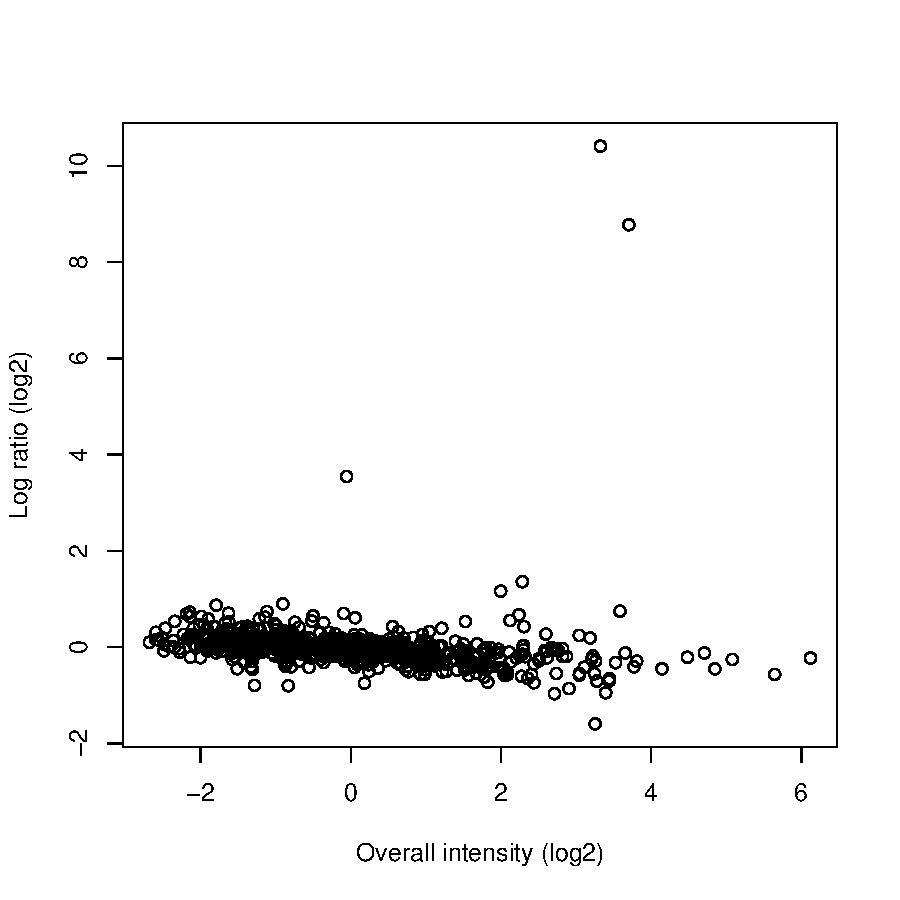
\includegraphics{rama-logratio}
\end{center}

Robustness is achieved by using a $t$-distribution for the errors
with a different degree of freedoms for each replicate array. This is formally equivalent to giving each replicate 
a different weight in the estimation process for each gene. A low number of degrees of freedom for one array will indicate that
the corresponding array contains numerous outliers. One could use the function {\tt hist} to look at the posterior mode 
of the degrees of freedom for each array.

\begin{center} 
\begin{Schunk}
\begin{Sinput}
> hist(mcmc.hiv$df[3, ], main = "Posterior degree of freedoms, array 3", 
+     xlab = "df", 50)
\end{Sinput}
\end{Schunk}
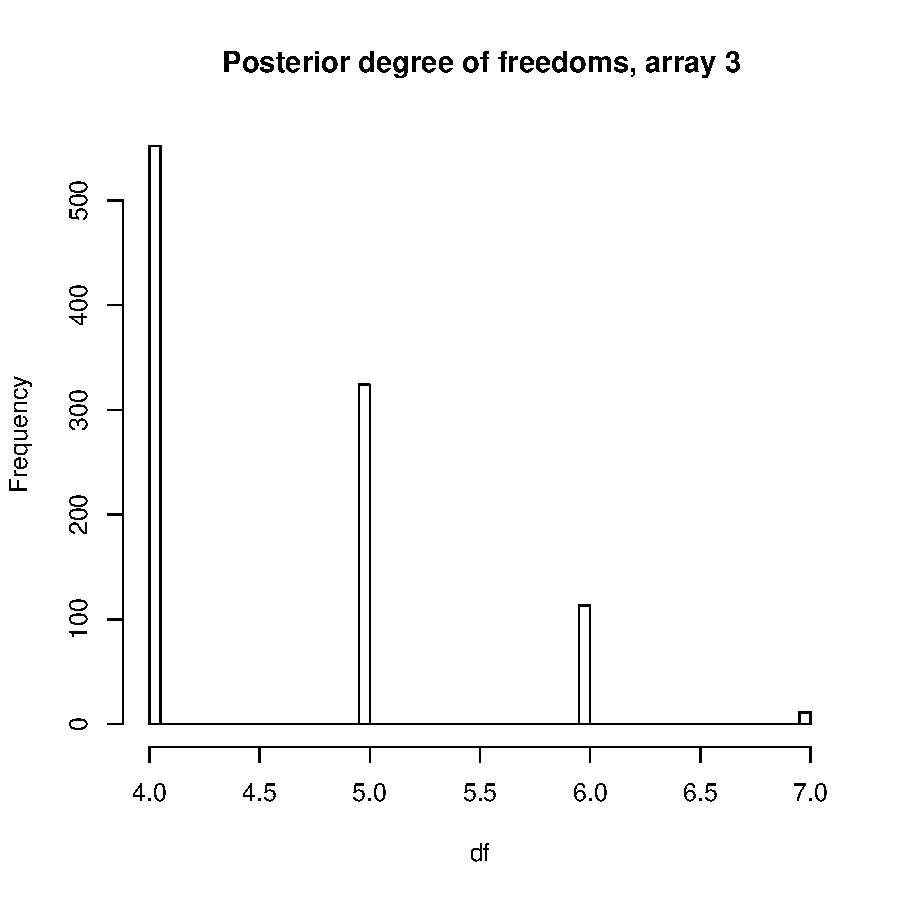
\includegraphics{rama-histdf}
\end{center}

Fitting a $t$-distribution can be seen as a weighted least square problem with a special hierarchical structure for the variances.
Similarly to a weighted least squares function, our function computes weights associated with each replicate. 
The weights can be useful as a tool for diagnosing the quality of the replicate measurements. If one knows the exact positions of the genes on the array, it 
is possible to look at the spatial variation of the weights. This can be done via the function {\tt weight.plot}.


Here is an example of such a plot:
\begin{center} 
\begin{Schunk}
\begin{Sinput}
> weight.plot(mcmc.hiv, hiv[1:640, 9:10], array = 3)
\end{Sinput}
\end{Schunk}
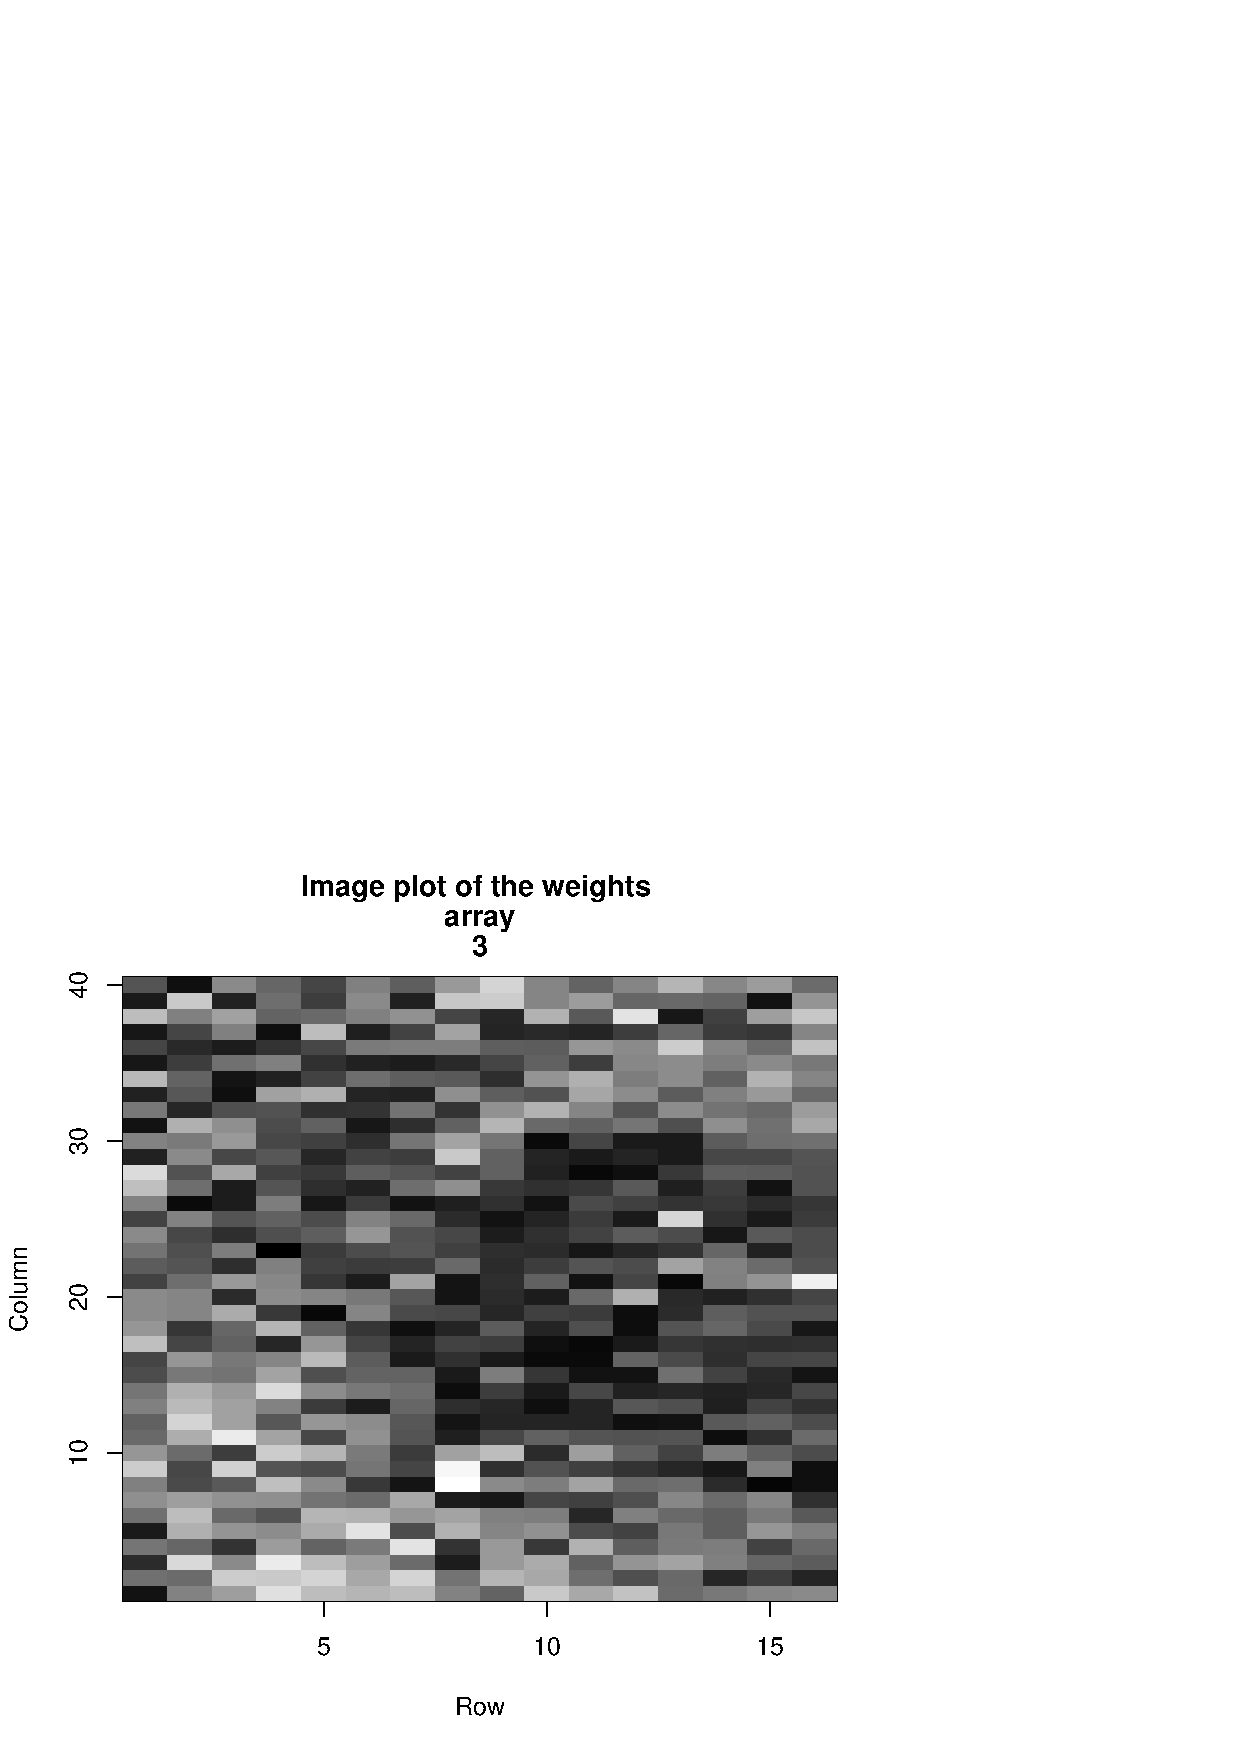
\includegraphics{rama-imagew}
\end{center}
Small weights, corresponding to light colors in the image plot, indicate  outliers. The image plot of the weights could be useful to detect 
possible artifacts or array outliers, \textit{etc}.   


\subsection{Estimating the shift}
The log transformation with shifted origin is often used in the context of gene expression data \cite{bib:kerr00,bib:cui02}.
One question is how to choose the shift, $\kappa$. 
We estimate the shift by fitting the same model as {\tt fit.model} with Gaussian sampling errors, constant variance and 
a vague uniform prior for $\kappa$. Then we use the posterior mean of $\kappa$ as a point estimate for the general model.


\begin{Schunk}
\begin{Sinput}
> mcmc.shift <- est.shift(hiv[1:640, c(1:4)], hiv[1:640, c(5:8)], 
+     B = 2000, min.iter = 1000, batch = 10, mcmc.obj = NULL, dye.swap = TRUE, 
+     nb.col1 = 2)
\end{Sinput}
\end{Schunk}

Note that the shift can also be estimated automatically with the {\tt fit.model} function (See above).

\subsection{Computing time and batch mode}

The computing time can be quite long depending on the number of genes and replicates. 
It takes about 5 hours to run the MCMC on the full HIV data set using a Linux machine with AMD Athlon at 2GHz. 
However we feel that this additional computational cost is 
worth the effort and can lead to some very good results. 
The code can be run in batch mode without any user intervention; this optimizes 
computing resources and allows the user to perform other tasks at the same time. 
R code can be run in batch mode by typing {\tt R CMD BATCH myfile.R} 
at the shell prompt. The file {\tt myfile.R} contains the command to execute.
An example file could be the following,
\begin{Schunk}
\begin{Sinput}
> library(rama)
> data(hiv)
> mcmc.hiv <- fit.model(hiv[, c(1:4)], hiv[, c(5:8)], B = 50000, 
+     min.iter = 5000, batch = 90, shift = 30, mcmc.obj = NULL, 
+     dye.swap = TRUE, nb.col1 = 2)
> save(mcmc.hiv, file = "mcmc.hiv.R")
\end{Sinput}
\end{Schunk}
Then, when the execution is done one can load the resulting output into R using the {\tt load} command. For further details about the {\tt BATCH} command type {\tt ?BATCH} in R.\\

\section{Acknowledgment}
This research was supported by NIH Grant 8 R01 EB002137-02.

%%%%%%%%%%%%%%%%%%%%%%%%%%%%%%%%%%%%%%%%%%%%%%%%%%%%%%%%%%%%%%%%%%%%%%%%%%%

\bibliographystyle{chicago}
\bibliography{robust_estimation} 

%%%%%%%%%%%%%%%%%%%%%%%%%%%%%%%%%%%%%%%%%%%%%%%%%%%%%%%%%%%%%%%%%%%%%%%%%%%

\end{document}
